\documentclass[8pt, a4paper]{article}
\usepackage{multicol}
\usepackage{listings}
\usepackage{geometry}
\usepackage{graphicx}
\usepackage{caption}
\usepackage{xstring}

\geometry{margin=0.3cm}
\graphicspath{{img}}

\pagenumbering{gobble}
\date{}

\lstdefinestyle{customstyle}{
  basicstyle=\ttfamily\scriptsize,
  breakatwhitespace=true,         
  breakautoindent=true,
  breaklines=true,                 
  captionpos=t,                    
  keepspaces=false,                 
  showspaces=false,                
  showstringspaces=false,
  showtabs=false,                  
  frame=single,
  stepnumber=1,                                           % the step between two line-numbers. If it's 1 each line will be numbered
  tabsize=2
  }

  \renewcommand\lstlistingname{}
  \DeclareCaptionFormat{listing}{}
  \captionsetup[lstlisting]{labelformat=empty}

  \newcommand{\lstinputwithcaption}[2]{%
    \lstinputlisting[caption={\texttt{#2}}]{#1}%
    }
    \newcommand{\codeListing}[6] {

      \begin{multicols}{2}
        \lstinputwithcaption{#1}{#2}

        \columnbreak

        \lstinputwithcaption{#3}{#4}

      \end{multicols}

      \begin{center}
        \includegraphics[scale=#5]{#6}
      \end{center}

      }

      \lstset{style=customstyle}

      \begin{document}

      NAMA: Radinal Shidiq Saragih

      KELAS: IF C 2023

      NPM: 5520123104

      \begin{enumerate}
        \item Bilangan Terbesar \& Terkecil

          \begin{multicols}{2}
            \begin{center}
            \lstinputwithcaption{./code/src/soal1/Main.java}{Main.java}
              
\includegraphics[scale=0.6]{S1.png}
            \end{center}
          \end{multicols}

        \item Penjumlahan \& Rata Rata Input

          \begin{multicols}{2}
            \begin{center}
              \lstinputwithcaption{./code/src/soal2/Main.java}{Main.java}
              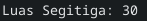
\includegraphics[scale=0.6]{S2.png}
            \end{center}
          \end{multicols}

        \item Floyd's Triangle

          \begin{multicols}{2}
            \begin{center}
              \lstinputwithcaption{./code/src/soal3/Main.java}{Main.java}
              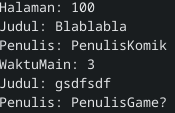
\includegraphics[scale=0.6]{S3.png}
            \end{center}
          \end{multicols}


        \item Penjumlahan Angka Ganjil

          \begin{multicols}{2}
            \begin{center}
              \lstinputwithcaption{./code/src/soal4/Main.java}{Main.java}
              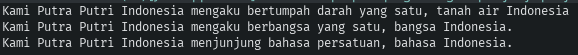
\includegraphics[scale=0.6]{S4.png}
            \end{center}
          \end{multicols}

        \item Segitiga Setengah dan Full

          \begin{multicols}{2}
            \begin{center}
              \lstinputwithcaption{./code/src/soal5/Main.java}{Main.java}
              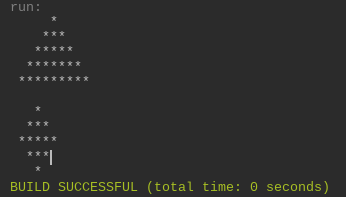
\includegraphics[scale=0.6]{S5.png}
            \end{center}
          \end{multicols}

        \item Tampilkan angka sebelas dua kali

          \begin{multicols}{2}
            \begin{center}
              \lstinputwithcaption{./code/src/soal6/Main.java}{Main.java}
              \columnbreak
              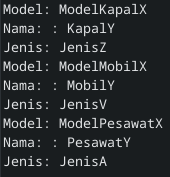
\includegraphics[scale=0.7]{S6.png}
            \end{center}
          \end{multicols}

        \item Perbedaan i++ dan ++i dengan while

          \begin{multicols}{2}
            \begin{center}
              \lstinputwithcaption{./code/src/soal7/Main.java}{Main.java}
              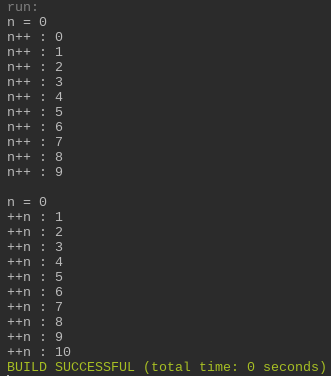
\includegraphics[scale=0.5]{S7.png}
            \end{center}
          \end{multicols}

        \item Perulangan Foreach

          \begin{multicols}{2}
            \lstinputwithcaption{./code/src/soal8/Main.java}{Main.java}
            \columnbreak
            \begin{center}
              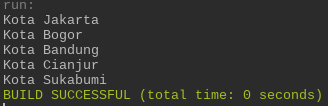
\includegraphics[scale=0.6]{S8.png}
            \end{center}
          \end{multicols}

      \end{enumerate}

    \end{document}
